%TODO 制作导航部分
\begin{withoutheadline}
\begin{frame}
\vspace*{-13mm}
\begin{figure}
	\hspace*{-4.2mm}
    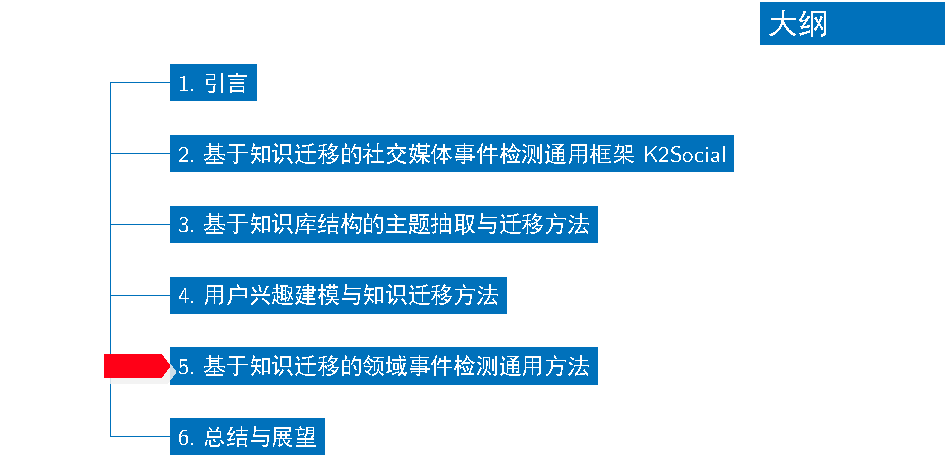
\includegraphics[width=1.0\paperwidth]{img/contents5_output.pdf}
\end{figure}

\end{frame}
\end{withoutheadline}

\section{基于知识迁移的领域事件检测通用方法}
%------------------------------
\begin{frame}
\frametitle{Motivation}
领域事件检测为什么是必须的?
\pdfnote{有什么合适的例子来说明领域事件检测呢?}
\end{frame}

%------------------------------
\begin{frame}
\frametitle{TaxoPhrase}	

\begin{figure}
	\caption{TaxoPhrase用于从维基百科知识库中抽取领域知识的示意图}
    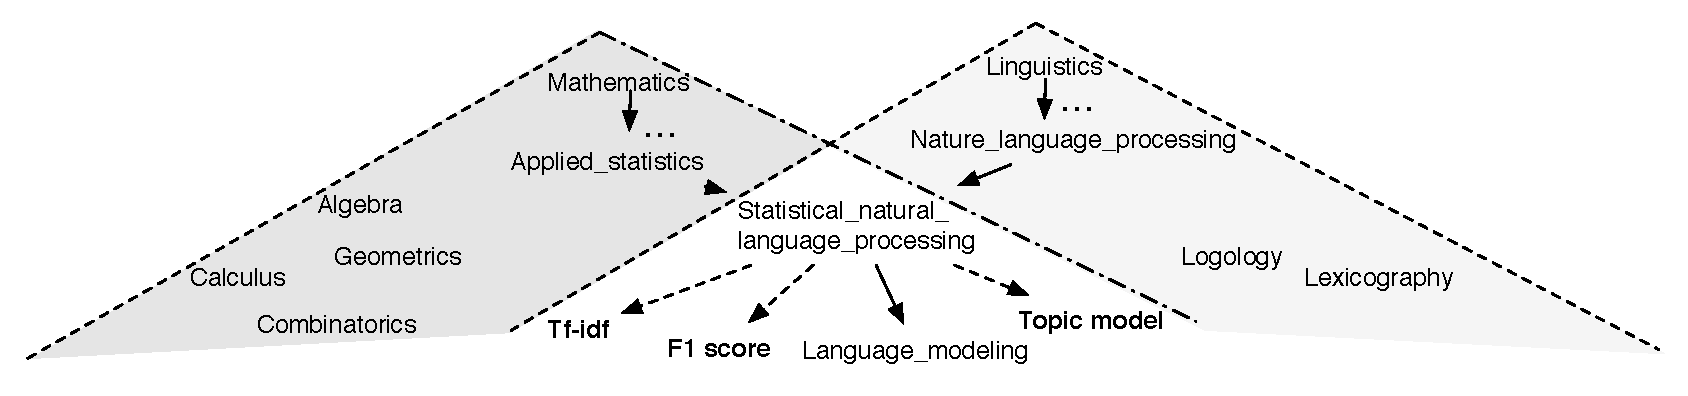
\includegraphics[width=1.0\textwidth]{img/TD+/taxophrase_motivation.pdf}
\end{figure}
\pdfnote{TaxoPhrase用于从知识库中抽取领域知识的示意图。用户1关心\textit{数学}领域中除\textit{统计自然语言处理}(白色区域)之外的知识(深灰色区域),用户2关心\textit{语言学}领域中除\textit{统计自然语言处理}之外的知识(浅灰色区域),在此场景中TaxoPhrase可将上述三部分用主题建模的方法加以探索与抽取。}
\end{frame}

